\documentclass[11pt,twoside]{article}
\usepackage[T1]{fontenc}
\usepackage[english]{babel}
\usepackage[utf8]{inputenc}

\usepackage{amsmath}
\usepackage{amscd}
\usepackage{amssymb}
\usepackage{tabularx}
\usepackage{url}
\usepackage{fancyhdr}
\usepackage[a4paper,margin=2.5cm,hmarginratio=1:1]{geometry}
\usepackage{graphicx}
\usepackage{pdfpages}
\usepackage{listings}

\title{Kometens Stoftsvans}
\author{Joakim Uddholm, juddholm@kth.se, 9110013290 \\
		Jo Tryti, tryti@kth.se, 8612050438}
\date{}

\begin{document}
\maketitle
\newpage
\includepdf[pages=22]{Lab3BuppgJO.pdf}

\section{Kometens bana}


Vår specifika komet banan fås utav ekv~\eqref{eq:kometens-elipse} och kan ses i Figure~\ref{fig:kometens-elipse}. Kometbanas figur är gjort med bibloteket matplotlib i python2. 
Vi deriverar även ekv~\eqref{eq:kometens-elipse} och får ekv~\eqref{eq:kometens-elipse-derivata} som senare kommer användas för beräkning av kometens riktnings vektor.

%Specifik elipse ekv
\begin{equation} \label{eq:kometens-elipse}
     r(\phi)=\frac{105}{1-0.4\cos\phi}
\end{equation}

\begin{equation} \label{eq:kometens-elipse-derivata}
    r'(\phi)=\frac{42}{(1-0.4\cos\phi)^2}
\end{equation}


\begin{figure}[h!] 
	\label{fig:kometens-elipse}
	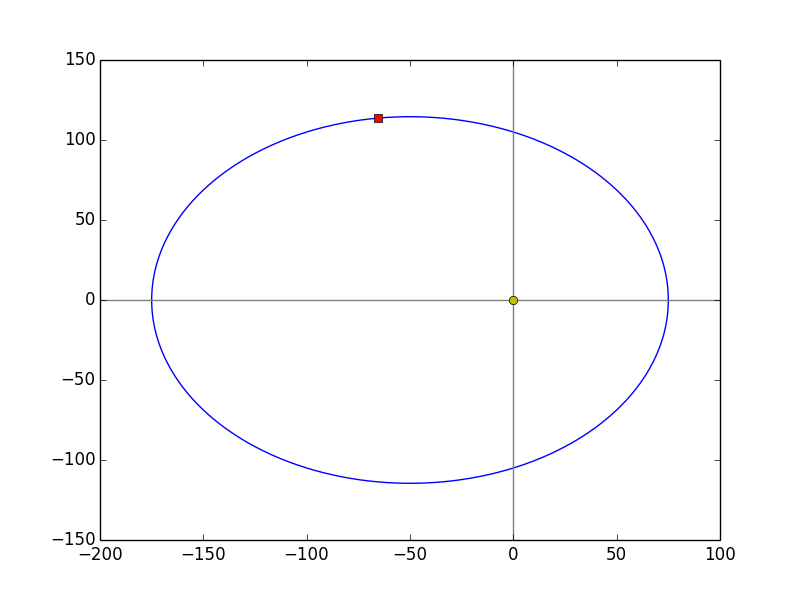
\includegraphics[width=300pt]{imgs/elipse.png}
  	\caption{Kometens bana med kometen utmarkerad vid vinkeln $2\pi/3$.}
\end{figure}

\section{Kometens riktning}
Med radien $r(\phi)$ fås en positionsvektor $P(\phi)$.
\begin{equation}
	P(\phi) = \begin{cases}
	x = r(\phi) cos(\phi) \\
	y = r(\phi) sin(\phi)
	\end{cases}
\end{equation}
Den partiella derivatan av ovanstående funktion ger riktningen $k$ som en funktion av $\phi$. 
\begin{equation}
	k(\phi) = \begin{cases}
	x = r'(\phi) cos(\phi) - r(\phi) sin(\phi) \\
	y = r'(\phi) sin(\phi) + r(\phi) cos(\phi)
	\end{cases}
\end{equation}

\section{Integrering för att lösa Differentialekvationen}
Vi använder RK4 (Runge-Kutta) för att lösa differentialekvationen och stega oss fram genom kometens bana. Med följande funktion kör vi genom Rk4. Notera att funktionen är oberoende av $t$. 
Vi har alltså ingen enhet för "tid".

\begin{lstlisting}
def _z_bis(z, t):
		x,y,dx,dy = z				
		d = -C / (sqrt(x**2 + y**2)**3)
		return [dx, dy, x * d, y * d]
\end{lstlisting}

Vid varje iteration av RK4 kommer $x$,$y$ ökas med $dx$,$dy$ och $dx$,$dy$ med $x*d$,$y*d$.

\section{Randvillkoret kometens hastighet}
För att få rätt bana på kometen och partiklarna måste vi bestämma kometens hastighet. Vi har redan riktningen i form av en vektor given tidigare ($r'(\phi)$), men vi behöver alltså längden av den vektorn.
Vi beräknar hastigheten genom att stegvis iterera fram via binärsökning för att försöka komma så nära $(75,0)$ som möjligt och en lite ful heuristik. Rimligtvist bör en för hög hastighet betyda att kometen skjuter förbi med högre $x$ värde när den passarerar $x$-axeln och på samma sätt bör en för låg hastighet innebära att kometen ligger närmare intill solen.
Vi ändrar alltså på hastigheten, kollar sedan hur långt ifrån den är ifrån sökta punkten och stegar sedan i riktning därifrån. Med varje steg delar vi på incrementet med 2. 

Följande dump visar varje iterationssteg. 
\begin{lstlisting}
[ 24.6713037   -0.19544714  -0.09545197  -0.24333948]
50.3286962951 -0.075 0.0125
[  5.73666559e+01  -3.98548466e-02  -2.14428638e-02  -1.57450197e-01]
17.6333441033 -0.0875 0.00625
[  7.96633416e+01  -4.90930107e-02   4.68889713e-03  -1.32294427e-01]
4.66334164463 -0.08125 0.003125
[  6.79726131e+01  -8.68044206e-02  -7.91303610e-03  -1.43959858e-01]
7.02738694136 -0.084375 0.0015625
[  7.36801153e+01  -7.73415211e-02  -1.50379723e-03  -1.37924404e-01]
1.31988472733 -0.0859375 0.00078125
[  7.66371476e+01  -8.23313732e-02   1.59731173e-03  -1.35061466e-01]
1.63714764788 -0.08515625 0.000390625
[  7.51498773e+01  -8.47663169e-02   4.74280680e-05  -1.36480625e-01]
0.149877275909 -0.084765625 0.0001953125
[  7.44127953e+01  -8.23038322e-02  -7.28084430e-04  -1.37199393e-01]
0.587204650506 -0.0849609375 9.765625e-05
[  7.47809355e+01  -1.54255630e-02  -2.50883694e-04  -1.36839293e-01]
0.219064481255 -0.08505859375 4.8828125e-05
[  7.49652266e+01  -5.02180537e-02  -1.01937831e-04  -1.36659776e-01]
0.0347733931075 -0.085107421875 2.44140625e-05
[  7.50574712e+01  -1.35807710e-01  -1.16059530e-04  -1.36570034e-01]
0.0574711685011 -0.0850830078125 1.220703125e-05
[  7.50113662e+01  -2.47242391e-02  -2.02045402e-05  -1.36614979e-01]
0.0113661787935 -0.0850708007812 6.103515625e-06
[  7.49882973e+01  -3.74702534e-02  -6.10607926e-05  -1.36637376e-01]
0.0117026967029 -0.0850769042969 3.0517578125e-06
[  7.49998320e+01  -3.10970230e-02  -4.06300695e-05  -1.36626177e-01]
0.000168031475695 -0.0850799560547 1.52587890625e-06
[  7.50055991e+01  -2.79105752e-02  -3.04166558e-05  -1.36620578e-01]
0.0055991305119 -0.0850784301758 7.62939453125e-07
[  7.50027156e+01  -2.95037852e-02  -3.55232003e-05  -1.36623377e-01]
0.00271556373373 -0.0850776672363 3.81469726563e-07
[  7.50012738e+01  -3.03004006e-02  -3.80765943e-05  -1.36624777e-01]
0.00127376968304 -0.0850772857666 1.90734863281e-07
[  7.50005529e+01  -3.06987109e-02  -3.93533218e-05  -1.36625477e-01]
0.000552869992248 -0.0850770950317 9.53674316406e-08
[  7.50001924e+01  -3.08978667e-02  -3.99916931e-05  -1.36625827e-01]
0.000192419480328 -0.0850769996643 4.76837158203e-08
[  7.50000122e+01  -3.09974448e-02  -4.03108806e-05  -1.36626002e-01]
1.21940577316e-05 -0.0850769519806 2.38418579102e-08

t = 1816
\end{lstlisting}

Det känns som att det borde finnas ett mer "matematiskt" sätt att beräkna detta. Tex med Newton-Raphson eller liknande. Vi får hur som helst ut värden på tiden $t$ och hastigheten $v$.

\section{Stoftpartiklarna}

Till slut använder vi samma funktioner för att stega genom Stoftpartiklarnas banor och plottar dem på samma figur. Vi behöver bara byta $C$ värden.
I figure är kryssen stoftpartiklarna. Man ser hur de avviker från kometens bana med olika banor beroende på $C$-värde. Stoftpartiklarna med $C$-värden mindre än 0 ser också
ut att vara utåtkrökta som enligt beskrivningen.

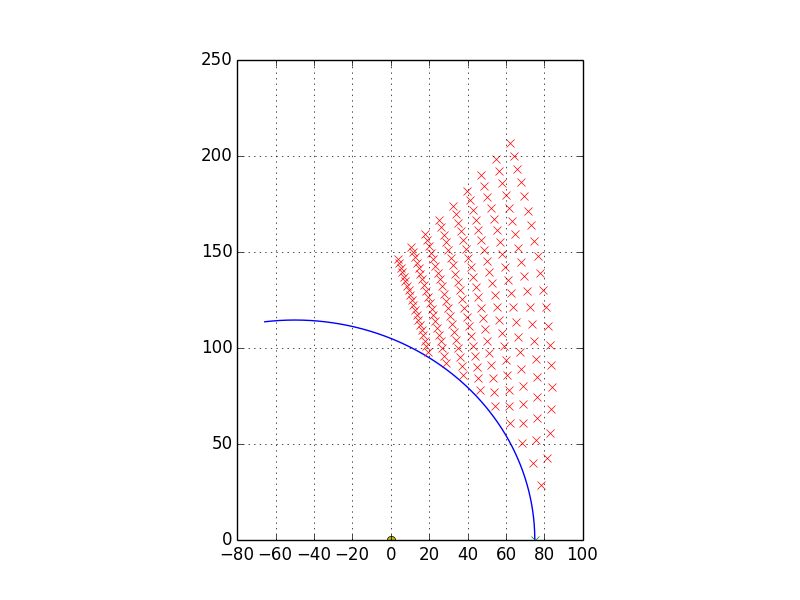
\includegraphics[width=300pt]{imgs/svans.png}

\end{document}
